

After two years of maintenance and upgrades, LHC started the second run phase, also known as \textit{Run2}, in 2015 featuring an increase of the center of mass energy up to 13\tev. The decision to begin the LHC’s second run at 13 TeV has been taken in order to optimize the delivery of particle collisions for physics research, and thereby speed the route to potential new physics. A conspicuous upgrade program has been planned also for the CMS ad ATLAS detectors, featuring the upgrades of many sub-detectors and software technicalities. While waiting for the first analysis results with 13\tev data, is possible to study the capabilities that searches for SUSY events in vector boson fusion events have using the brand new hardware and software setup. This chapter gives details on the sensitivity study of a SUSY VBF search performed using 2015 Monte Carlo simulated data.

\section{Signal and background samples}

The signal event samples are generated with the \texttt{MadGraph v5.2.1} program \cite{Alwall:2011uj}, considering pair production of gauginos with two associated partons. The signal events are generated requiring a pseudorapidity gap $|\deltaeta| > 4.2$ between the two partons, with $\pt > 30\gev$ for each parton. Signal cross sections are calculated at leading order using the MadGraph generator. The range of signal cross sections is $3$ fb for \charginopm = \neutralinotwo masses of 100, 200 and 300\gev and \neutralinoone mass of 0 nad 50\gev, for a total of six different benchmark points.

The Montecarlo background events used in for this study refers to the production run labeled as \textit{RunIISpring15MiniAODv2} and incorporate the \texttt{CTEQ10} \cite{Dulat:2013hea} parton distribution functions (PDF).The \texttt{POWHEG} and \texttt{MadGraph} generators are interfaced with the \texttt{PYTHIA v8.5.12} \cite{Sjostrand:2006za} program, which is used in the mathing between the matrix elements and the parton shower, and the hadronization processes. 

All the Monte Carlo samples are store in a new format called \texttt{miniAOD} \cite{bib:WorkBookMiniAOD}. This format is an updated version of the previously used one in order to account new CMS reconstruction features, between the time of the original proposal and the starting of Run2. A comprehensive list of all the samples used in this study il listed in \autoref{sec::sampleslist_13tev}.

\section{Object reconstruction}

During the technical stop the experiment underwent through several updates on both hardware and software side. This	translates also into an updated version of the physical object definition used for this study with respect to the one used in the 8\tev analysis.

The \hadtau object reconstruction went through a major update with the introduction of new isolation and decay mode discriminators and electron veto \cite{bib:TauID_13tev}. The new \hadtau object reconstruction has been commissioned for $\pt > 20$\gev ad in all $\eta$ ranges. By using the specifications suggested by the Tau POG there's an increase of the overall TauID efficiency of about 10\% for loose isolated \hadtau with respect to the 8\tev specifications, going up to 71\% for $Z \longrightarrow\tau\tau$ events\cite{bib:TauID_13tev}. A detailed list of the \hadtau object selection can be found on Table \ref{table:tauobjdefinition_13TeV}. 

The Jet object definition remained unchanged.  

With Run 2 the experiment will gain access to a new trigger list. The aim is to use a trigger that is exclusively making an online selection on the di-jet object kinematic properties. Differently with the 8\tev trigger version this trigger can't be seeded by a level one trigger based on \met. The drop of all online selections over the \hadtau properties leads to some important advantages Firstly it is possible to have a lower \hadtau \pt selection. Secondly it is possible to go from a 1-prong to a 3-prong decay selection since this stringent requirement is not part anymore of any level 1 trigger seed. 

The b-tag object reconstruction has now an updated discriminator as suggested by the POG \cite{bib:BJetID_13tev}.

\section{Cross section limit studies}

The aim of this study is to optimize the event cuts is order to exclude signal at the lowest cross section measurable. A cross section limit is made my setting the significance $\alpha$ to:

\begin{equation}
\alpha = 2
\label{eq::significance_xsec_limit}
\end{equation}

There are several however definitions of significance $alpha$ available in literature. The one picked for this 13\tev study is a frequentist definition based on completely standard concepts\cite{Punzi:2003bu} is generally applicable, and has a very clear interpretation. It is particularly suitable for optimization, being independent of a-priori expectations about the presence of a signal, thus allowing the determination of a single set of cuts that is optimal both for setting limits and for making a discovery. The definition of sensitivity is:

\begin{equation}
\alpha = \dfrac{S}{\dfrac{a}{2} + \sqrt{B + (0.5 \cdot B)^{2}}}
\label{eq::punzi_formula}
\end{equation}

with $a$ as the confidence level expressed in terms of $\sigma$, $S$ and $B$ are respectively the number of signal and background vents for a given selection. One of the most important features of \autoref{eq::punzi_formula} is non-diverging in case of $B = 0$.

The number of signal events can be defined as:

\begin{equation}
S = \epsilon \cdot \sigma_{sec} \cdot L
\label{eq::punzi_signal_events}
\end{equation}

with $\epsilon$ as the efficiency for a given selection criteria, $\sigma_{sec}$ as the cross section of the signal process considered and $L$ and the luminosity given by the experiment. Is it possible now to define the efficiency $\epsilon$ as function of variables used in the analysis event selection. Three of the most important variables in the 8\tev analysis has been chosen for this study: $\pt(\hadtau)$,\met and $m_{jj}$. The definition of $\epsilon$ given in \autoref{eq::punzi_signal_events} now becomes:

\begin{equation}
\epsilon^{signal} ( \pt(\hadtau) , m_{jj} ,  \met ) = \dfrac{N^{signal}_{passed}(\pt(\hadtau) , m_{jj} ,  \met)}{N^{signal}_{total}}
\label{eq::punzi_efficiency}
\end{equation}

with $N^{signal}_{passed}$ as the number of signal events passing the selection criteria as function of the chosen variables and $N^{signal}_{total}$ as the number of total signal events. Is easy to notice that by fixing the significance value as shown on \autoref{eq::significance_xsec_limit} the cross section $\sigma_{sec}$ in \autoref{eq::punzi_signal_events} becomes indeed the cross-section limit $\sigma^{lim}_{sec}$. After merging both \autoref{eq::punzi_signal_events} and \autoref{eq::punzi_efficiency} the cross section limit $\sigma^{lim}_{sec}$ is defined as:
	
\begin{equation}
\sigma^{lim}_{sec}( \pt(\hadtau) , m_{jj} ,  \met ) = \dfrac{\alpha \cdot\left(\dfrac{a}{2} + \sqrt{B( \pt(\hadtau) , m_{jj} ,  \met ) + (0.5 \cdot B( \pt(\hadtau) , m_{jj} ,  \met ))^{2}}\right)}{\epsilon^{signal} ( \pt(\hadtau) , m_{jj} ,  \met ) \cdot L}
\label{eq::xsec_lim}
\end{equation}



\subsection{Event selection}
\label{subsec::event_sel_13tev}

The values for $\epsilon^{signal}$ and $B$ are directly taken from the signal and background samples listed in \autoref{sec::sampleslist_13tev} after applying the event selection. The idea of this 13\tev study is to be as close as possible to the one done in 8\tev, therefore the event selection is the same as described in \autoref{sec:eventselection} with a few updates included.

As previously mentioned the event selection for this study is a function of the reconstructed tau $pt(\hadtau)$,\met and the di-jet candidate invariant mass $m_{jj}$, therefore those cuts are considered as free variables in the event selection. 

The uncertainties on the official 13\tev trigger list and on how good are those triggers simulated in Monte Carlo lead to the decision of removing the trigger requirement in the event selection. In case this study will use 13\tev data is useful to notice that a choice of a VBF-selection-seeded trigger will lead to an online selection over the di-jet canditates invariant mass $m_{jj}$.

Thanks to the improvements done in the \hadtau object reconstruction is now possible to include three-prong decaying taus in the event selection.

The di-jet \deltaeta cut has been removed due to its strong correlation to the di-jet canditates invariant mass $m_{jj}$ as shown in the 8\tev study \cite{Khachatryan:2015kxa}.

For better visualization and understanding all the selection criteria are summarized the following way:

\begin{itemize}
	\item \textbf{Central selection}
	\begin{itemize}
		\item two three-prong hadronically decaying $\tau$ with variable $\pt$
		\item $\met = \text{variable}$
		\item at least two jets with $p_{T}^{jet}\geq30~$\gev, $|\eta_{jet}|\leq5$ and loose jetID
		\item $\Delta R(jet,\tau)\geq0.3$
		\item b-tag veto
	\end{itemize}
	\item \textbf{VBF selection}
	\begin{itemize}
		\item $sign(\eta^{jet 1}\cdot\eta^{jet 2})==-1$
		\item $\mjj = \text{variable}$
	\end{itemize}
\end{itemize}

\subsection{Background estimation}

Similarly to the analysis at 8\tev, the hardest challenge for this study is to determine the number of background events in the signal region. As described in \autoref{sec::bg_contributions}, the main background contribution is coming from QCD events. The remaining background contributions are considered negligible. Even though this study is characterized by a loosening of the selection cuts with respect to the previous analysis, the limited statistics of the used Monte Carlo samples gives a very scarce number of selected events. The problematic of a limited statistics is solved by estimating the number of background events in the signal region through a two-fold ABCD method. It involves the usage of two distinct correction factors in order to gradually convert the number of background events, taken from a starting control region with looser cuts, into the signal region ones. This method is defined under the same assumptions made for the 8\tev analysis, listed in \autoref{sec:bgestimation}.

With the idea in mind of developing a method similar to the one used for 8\tev, the regions are defined by two distinct variables: the isolation of the di-tau candidates and the inversion of the VBF cuts. Three are the regions defined in purpose of this method. The signal region, also called SR, is defined as the region fulfilling all the cuts listed in \autoref{subsec::event_sel_13tev}. Control region two, also called CR2, has the same selection as the one for the signal region but requires the inversion of the VBF-related cuts. Finally control region tree, also called CR3, has the same selection as CR2 but requires the di-tau candidates to have a Loose isolated and a non-isolated \hadtau.

As previously mentioned two are the conversion factors used in this method. The first factor, named "\textit{NL-to-2T}" or "\textit{None-Loose to two Tight}", allows to convert the number of selected events from CR3 to CR2. This factor is derived from a study over the same QCD sample where the event population is high by only requiring at least four reconstructed jets in the event and is defined as:

\begin{equation}
\text{NLto2T} = A * B
\end{equation}

where $A$ and $B$ are ration. Going further in details $A$ has as denominator the number of events with at least four jets where at least one fo these jets is matched with a loose isolated \hadtau. In case this matched \hadtau is also tight isolated the events is counted in the numerator:

\begin{equation}
A = \dfrac{N_{events}(\text{the matched }\hadtau\text{ is also tight isolated })}{N_{events}(\leq 1\text{jet matched to loose }\hadtau)}
\end{equation}

The definition of $B$ is equal to $A$ with the only difference that the \hadtau matched to a jet in the denominator is non-isolated:

\begin{equation}
B = \dfrac{N_{events}(\text{the matched }\hadtau\text{ is also tight isolated })}{N_{events}(\leq 1\text{jet matched to non-isolated }\hadtau)}
\end{equation}

The second conversion factor is identical to the VBF conversion factor defined in \autoref{sec:bgestimation} with the only difference of the updated version of the VBF cuts for the 13\tev study:

\begin{equation}
\text{VBF} = \frac{\epsilon^{QCD}_{VBF}}{1 - \epsilon^{QCD}_{VBF}}
\end{equation}

where $\epsilon^{QCD}_{VBF}$ is previously defined in \autoref{eq:vbfeff}. 

Finally the number of predicted events in the signal region is:

\begin{equation}
B = N^{QCD}_{SR} = N^{MC}_{CR3}  \cdot \text{NLto2T} \cdot \text{VBF}
\label{eq::qcdbgpred_13tev}
\end{equation}

A representation of the regions and the conversion factor used in this two-fold ABCD method is shown in \autoref{fig:crs_13tev}.

\subsection{Systematic and statistical uncertainties}

Similarly to how is done for the 7\tev analysis, two different sources of systematics has been taken into account for this study. 

The first source is the uncertainty over the Monte Carlo sample production. Following the strategy used in the previous analysis this statistical uncertainty is estimated by the variation on the cross-section limit result after considering a $\pm 50\%$ variation of the Monte Carlo statistics.

The second source of the uncertainty is the instability on the VBF efficiency $\epsilon^{QCD}_{VBF}$ over different \hadtau isolation region. Again this uncertainty is calculated by taking into account the maximal variation of the VBF conversion factor in the previously define control regions, CR2 and CR3.

\section{Results}

The definition of the cross-section limit $\sigma^{lim}_{sec}$, as given in \autoref{eq::xsec_lim}, allows the scan in a three-dimensional space defined by the variables $\pt(\hadtau)$ , \mjj and \met. The minimum cross-section limit found by the scan gives the optimal event selection cuts for each of the available signal benchmark points. The distribution of the most important analysis variables are shown in \autoref{fig::crplots1_Taui2TightIso_13tev_results} and \autoref{fig::crplots2_Taui2TightIso_13tev_results}; for this purpose the cuts over the study variables $\pt(\hadtau)$, \mjj and \met have been removed. 

In order to achieve a better reading over the results of the cross-section limit study it is possible to simplify the three-dimensional problem in a "\textit{two plus one}" dimensional one. Following this approach the cross-section limits are calculated and shown in a two-dimensional plot defined in bins of \mjj and \met, the process is repeated for each of the chosen $\pt(\hadtau)$ cuts.

\begin{figure}[tbh!]
	\centering
	\begin{tabular}{cc}
		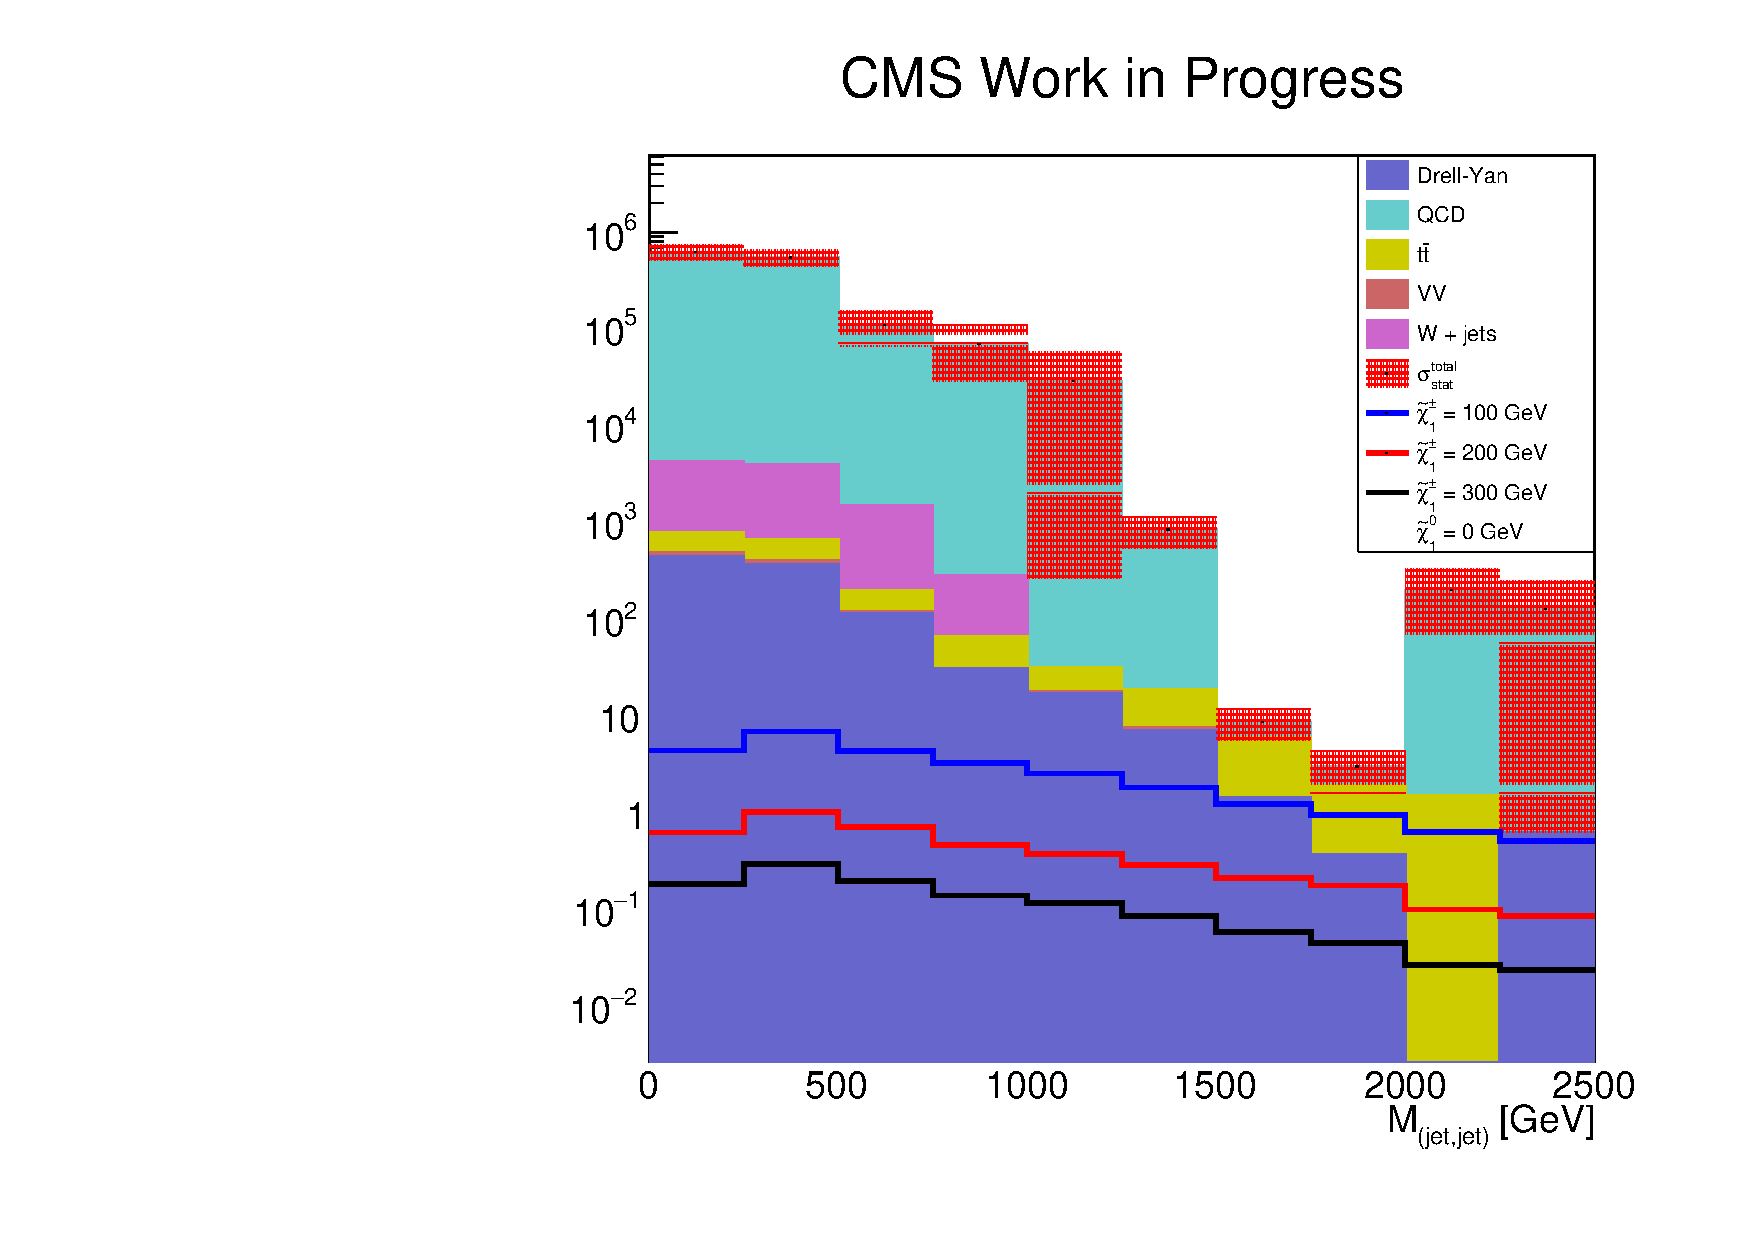
\includegraphics[width=0.5\textwidth]{analysis/pics/h_dijetinvariantmass_Taui2TightIso.pdf}
		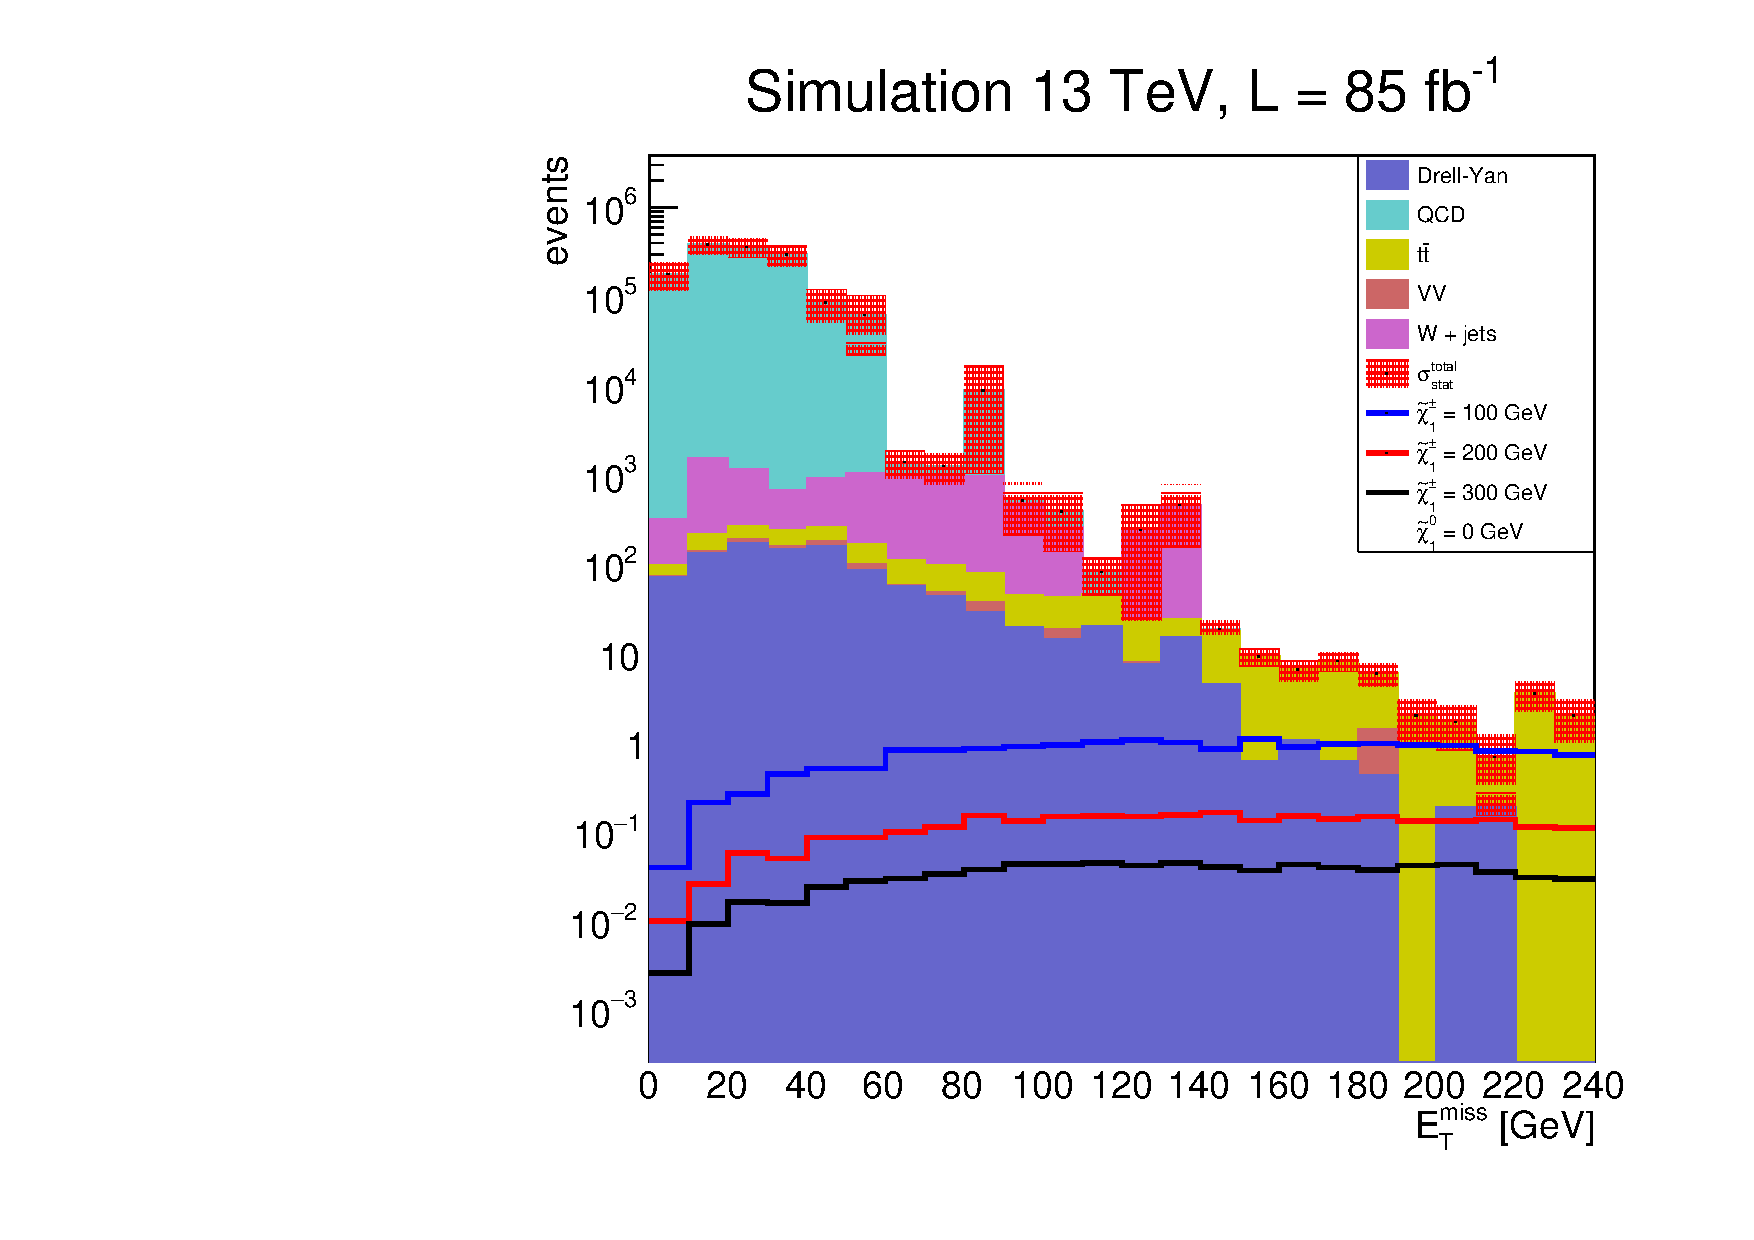
\includegraphics[width=0.5\textwidth]{analysis/pics/h_met_Taui2TightIso.pdf} 		
	\end{tabular}
	\caption{(Left) Di-jet invariant mass distribution and (Right) and \met distribution of selected signal and all MC background samples in signal region.}
	\label{fig::crplots1_Taui2TightIso_13tev_results}
\end{figure}

\begin{figure}[tbh!]
	\centering
	\begin{tabular}{cc}
		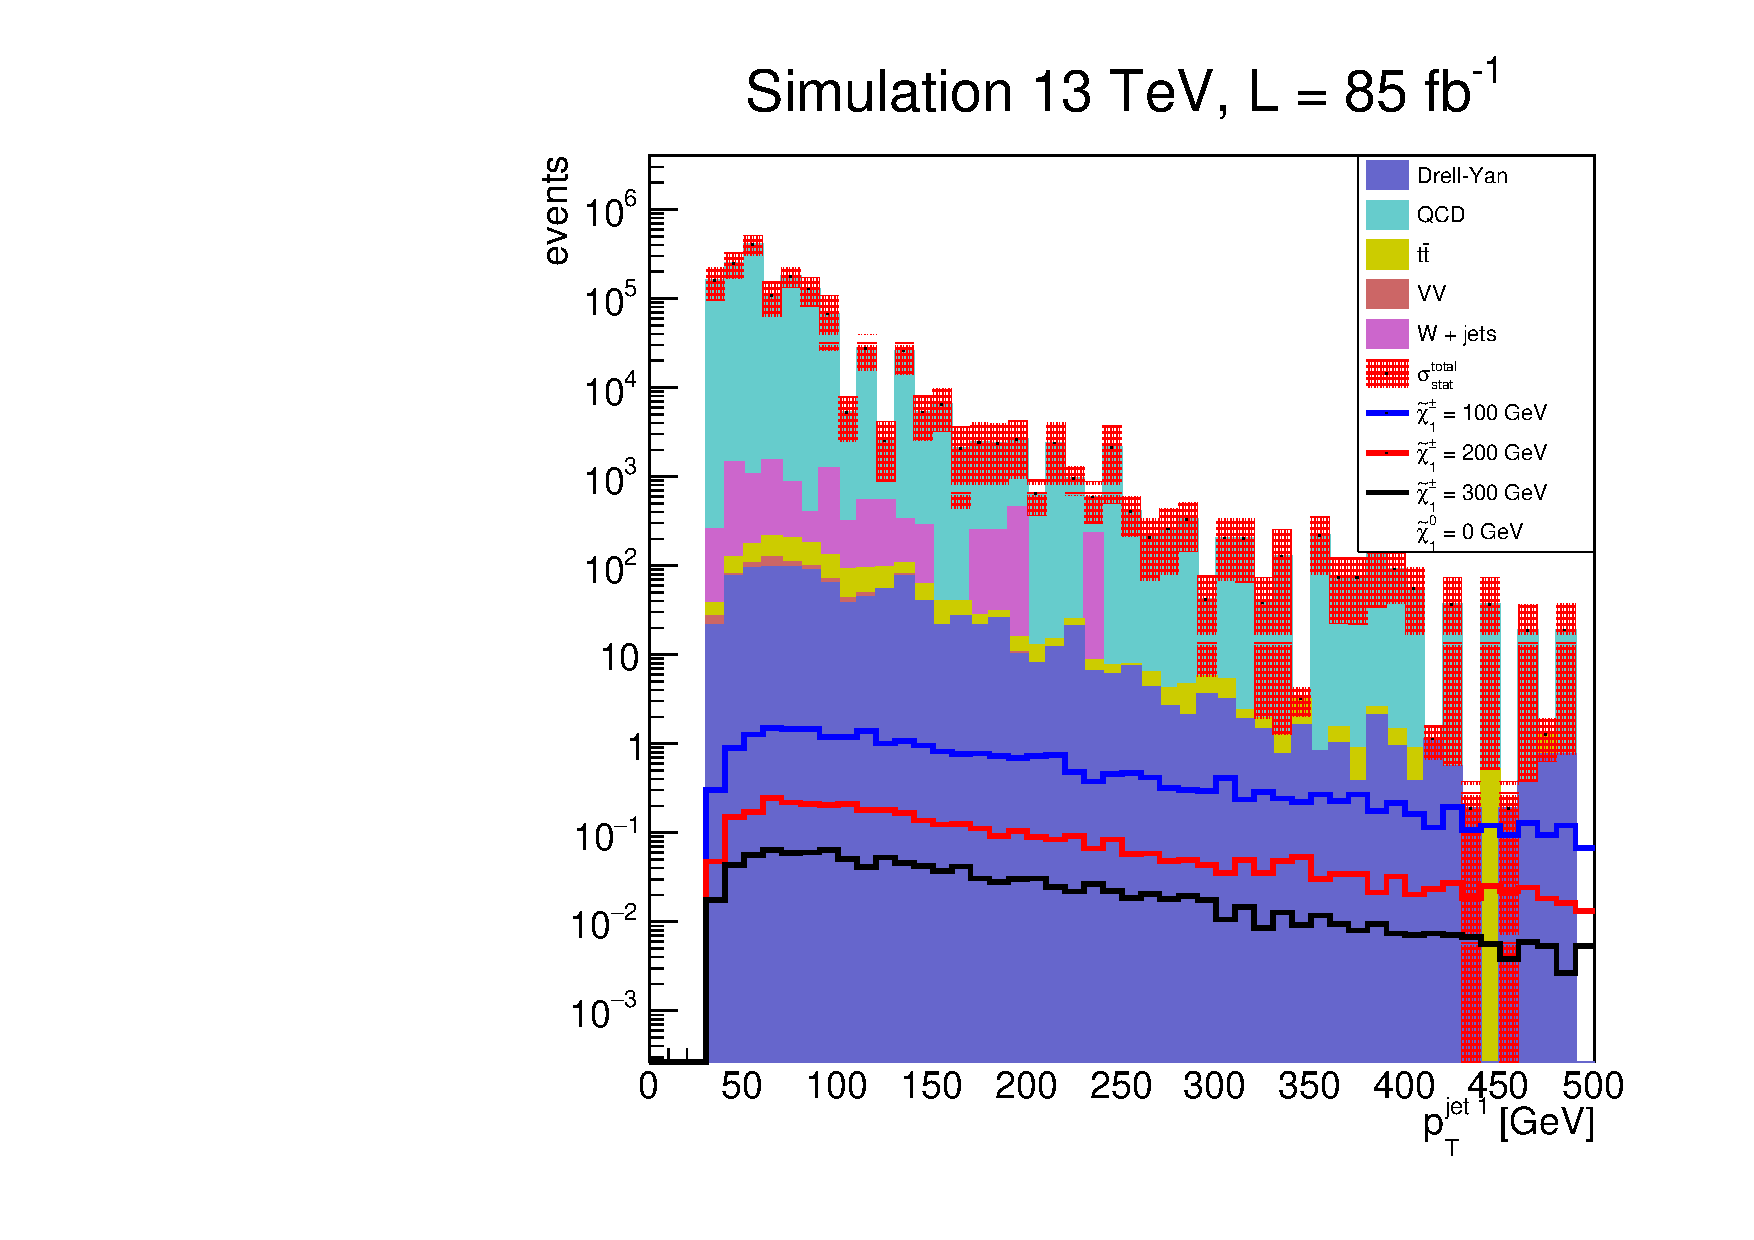
\includegraphics[width=0.5\textwidth]{analysis/pics/h_jet1pt_Taui2TightIso.pdf}
		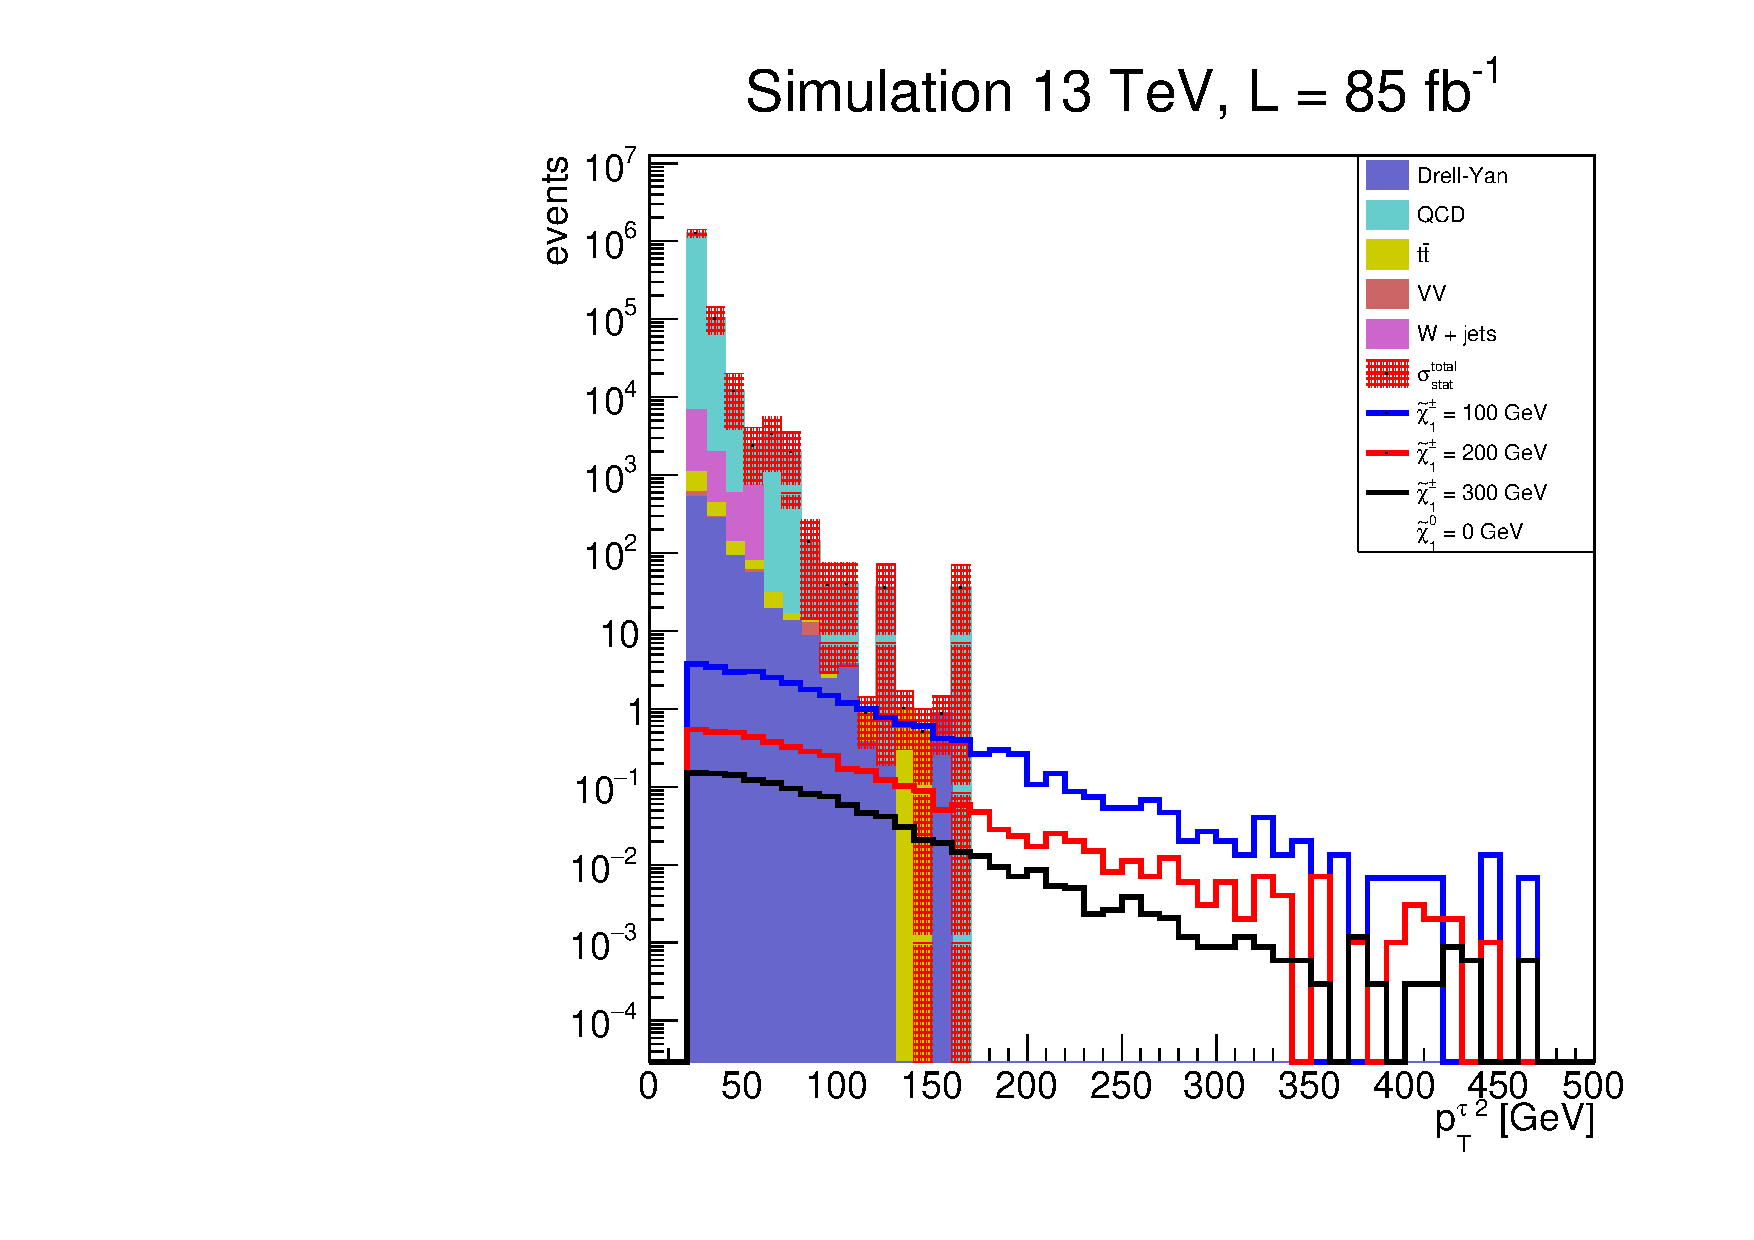
\includegraphics[width=0.5\textwidth]{analysis/pics/h_tau2pt_Taui2TightIso.pdf} 		
	\end{tabular}
	\caption{(Left) Leading jet \pt distribution and (Right) and second leading \hadtau \pt distribution of selected signal and all MC background samples in signal region.}
	\label{fig::crplots2_Taui2TightIso_13tev_results}
\end{figure}


Each of the two-dimensional bins stores a $\sigma^{lim}_{sec}$ for the given $\pt(\hadtau)$ , \mjj and \met cuts setup. The most important input values to \autoref{eq::xsec_lim} are the signal efficiency $\epsilon^{signal}$, as defined in \autoref{eq::punzi_efficiency},  and the number of predicted background events $B$, as defined in \autoref{eq::qcdbgpred_13tev}. The remaining input values are the luminosity $L$ and the confidence level $a$. The predicted luminosity for the 13\tev Run \cite{Bruning:2002yh} is estimated between 75 and 100 \invfb; for the purpose of this study its value has been set to $L = 85\invfb$. The corresponding value in terms of $\sigma$ to a confidence level of 95\%  is $2.5$.

A full list of the study results is given in \autoref{sec::xseclim_results}. The high impact of the $\pt(\hadtau)$ cut over the signal efficiency $\epsilon^{signal}$ is visible, accordingly to what was also shown in the 8\tev analysis. Also important to mention that the cross section limits increases with the increasing \charginopm, \neutralinotwo and LSP masses. Therefore the best cross-section limit scenario is given for a \charginopm and \neutralinotwo mass of 100\gev, a massless LSP and a $\pt(\hadtau)$ cut of 20\gev as shown on \autoref{fig::xsec_lim_selected_results}. The left picture shows the overall cross-section limit map study, the one on the right shows a magnification of the most interesting area. The cross-section limit minimum is:

\begin{equation}
\sigma_{lim}^{min}\pm(stat.)\pm(MC syst.)\pm(VBF syst.) = 0.0327\pm0.0068^{+0.0031+ 0.0011}_{-0.0036-0.0005} [\text{pb}]
\label{eq::xsec_lim_best_result}
\end{equation}

for the optimal cuts of  $\pt(\hadtau) <  20$,  $ \mjj< 250 $ and $\met < 130$.

\begin{figure}[tbh!]
	\centering
	\begin{tabular}{cc}
		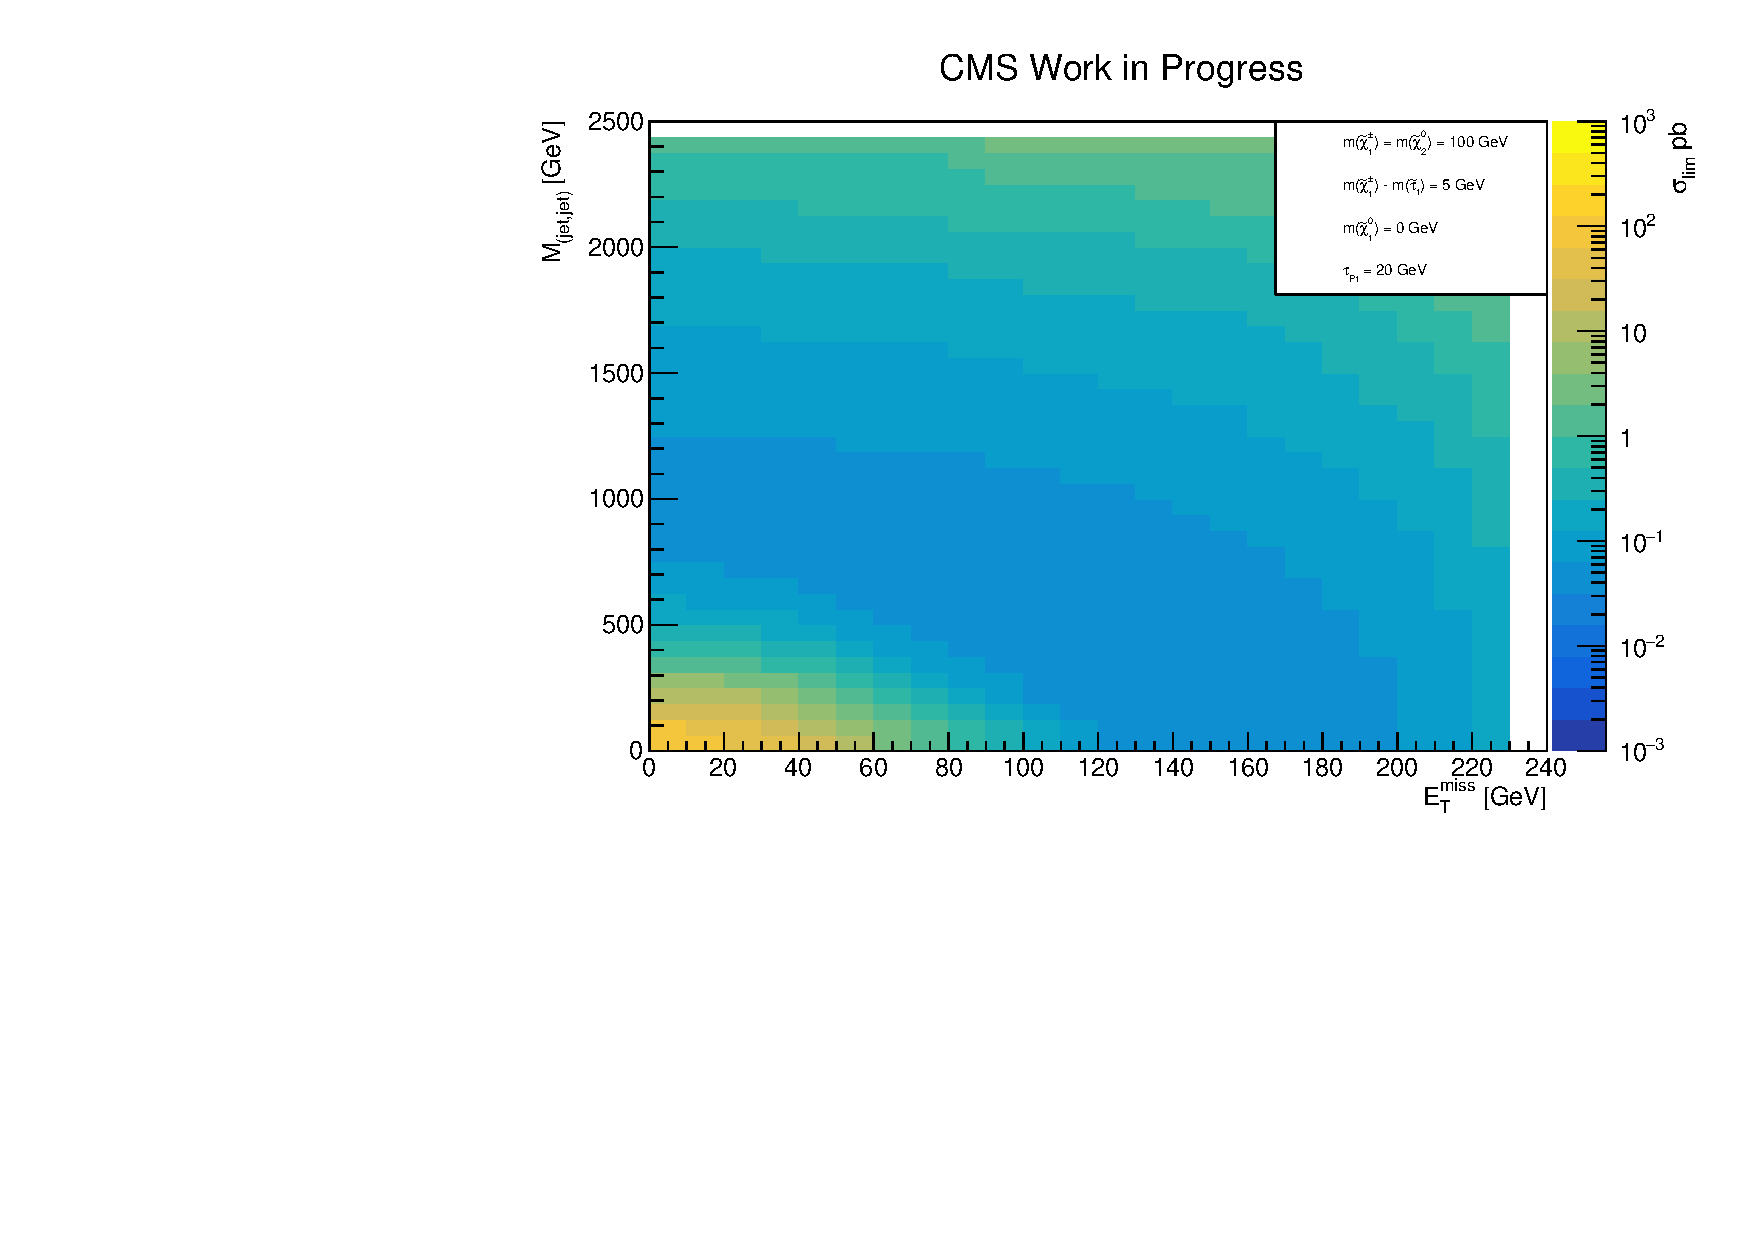
\includegraphics[width=0.45\textwidth]{analysis/pics/JetInvMass_vs_MET_xsec_chi100_lsp000_taupt20.pdf}
		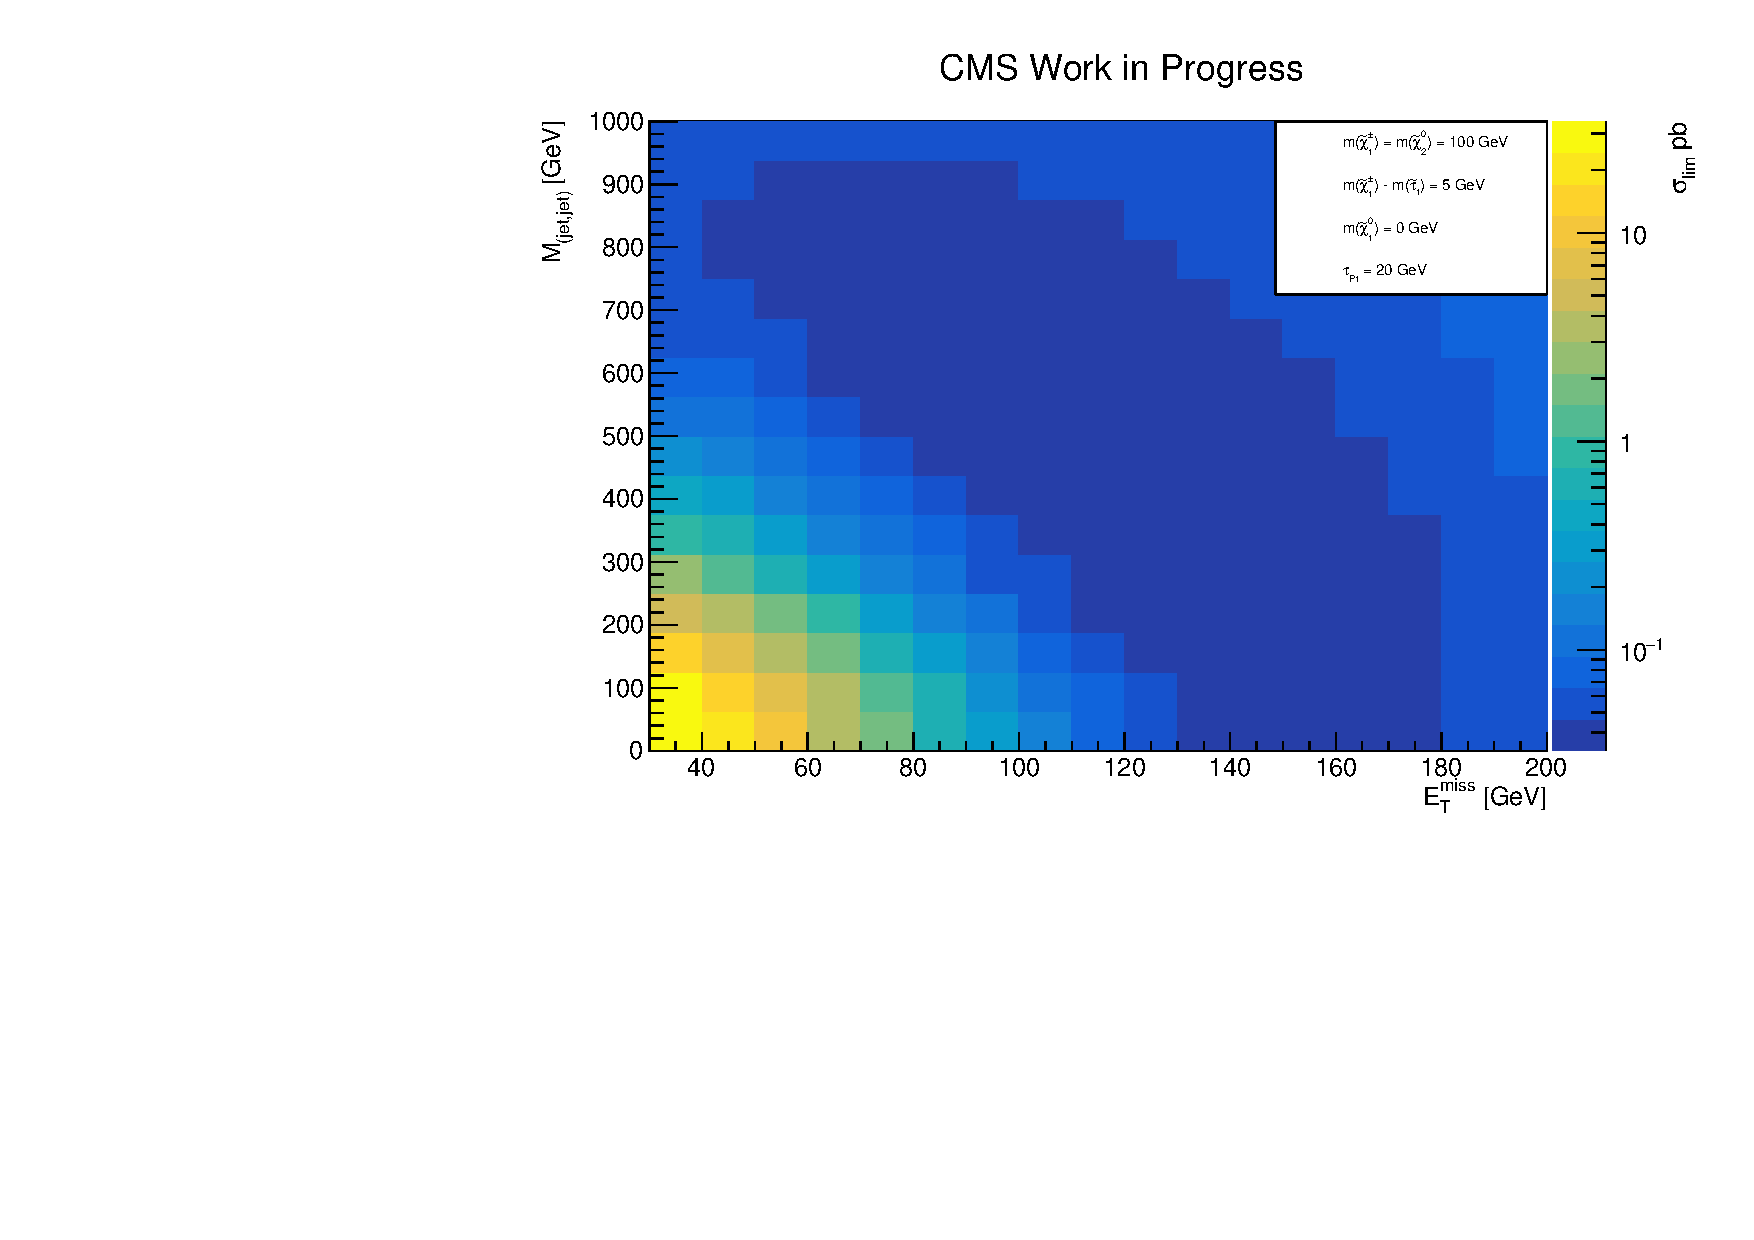
\includegraphics[width=0.45\textwidth]{analysis/pics/JetInvMass_vs_MET_xsec_chi100_lsp000_taupt20_zoom.pdf} 		
	\end{tabular}
	\caption{(Left) Cross section limit as function of $m_{jj}$ and \met for \charginopm = \neutralinotwo = 100 GeV, \neutralinoone = 0 GeV and an offline selection on $\pt(\hadtau) <  20\gev$. (Right) Zooming into the minimum cross section limit area for the same benchmark point.}
	\label{fig::xsec_lim_selected_results}
\end{figure}

By comparing the 7\tev cross-section limit values with the ones at 13\tev is possible to see that the previous analysis performs better in terms of limit setting as shown in \autoref{table::xseclim_7tev13tev_comparison}. The high statistical and systematic uncertainties shown in the 13\tev is caused by the cut over the $\pt(\hadtau)$, which dramatically reduces the QCD statistics. Is worth to mention however that the 7\tev analysis has a selection which in general prevents the comparison in areas of the previously defined three-dimensional phase-space where the 13\tev analysis is meant to perform better.

\begin{table}
\begin{center}
\begin{tabular}{| c | c | c | }
	\toprule
	\multicolumn{3}{| c | }{For $\pt(\hadtau) <  45\gev$  $\met > $ 30, $\mjj>250~$\gev, m(\neutralinoone) = 50\gev} \\
	\midrule
	m(\charginopm) = m(\neutralinotwo)  & $\sigma_{lim}^{min}\pm(stat.)\pm(syst.)$ [pb] (8\tev) & $\sigma_{lim}^{min}\pm(stat.)\pm(syst.)$ [pb] (13\tev)\\
	\midrule
   100\gev &  $0.084\pm0.016^{+0.18}_{-0.01}$ & $0.60\pm0.69^{+1.62}_{-0.87}$  \\
   200\gev &  $0.14\pm0.02^{+0.03}_{-0.04}$ & $0.65\pm0.74^{+1.74}_{-0.94}$ \\
   300\gev &  $1.43\pm0.52^{+0.49}_{-0.38}$ & $1.19\pm1.39^{+3.2}_{-1.71}$  \\
	\bottomrule
\end{tabular}\caption{Cross-section limit comparison between the 8\tev analysis and the 13\tev sensitivity study. The chosen values corresponds to an identical selection and signal benchmark points. Cross section limit minimum reached at the given cuts for $\pt(\hadtau) <  45\gev$  $\met > $ 30, $\mjj>250~$\gev, m(\neutralinoone) = 50\gev.}
\label{table::xseclim_7tev13tev_comparison}
\end{center}
\end{table}

A comparison between the cross-section limit values coming from this study and the cross-section limit granted by the CMS collaboration \cite{bib:SUSYCrossSections13TeVn2x1wino_13tev} is shown in \ref{fig:xsec_confront_13tev}. The final result coming from this 13\tev study shows the capability, within the statistical uncertainty, that this analysis topology has in searching for SUSY scenarios with light electroweakinos.

\begin{figure}[tbh!]
	\centering
	\begin{tabular}{cc}
		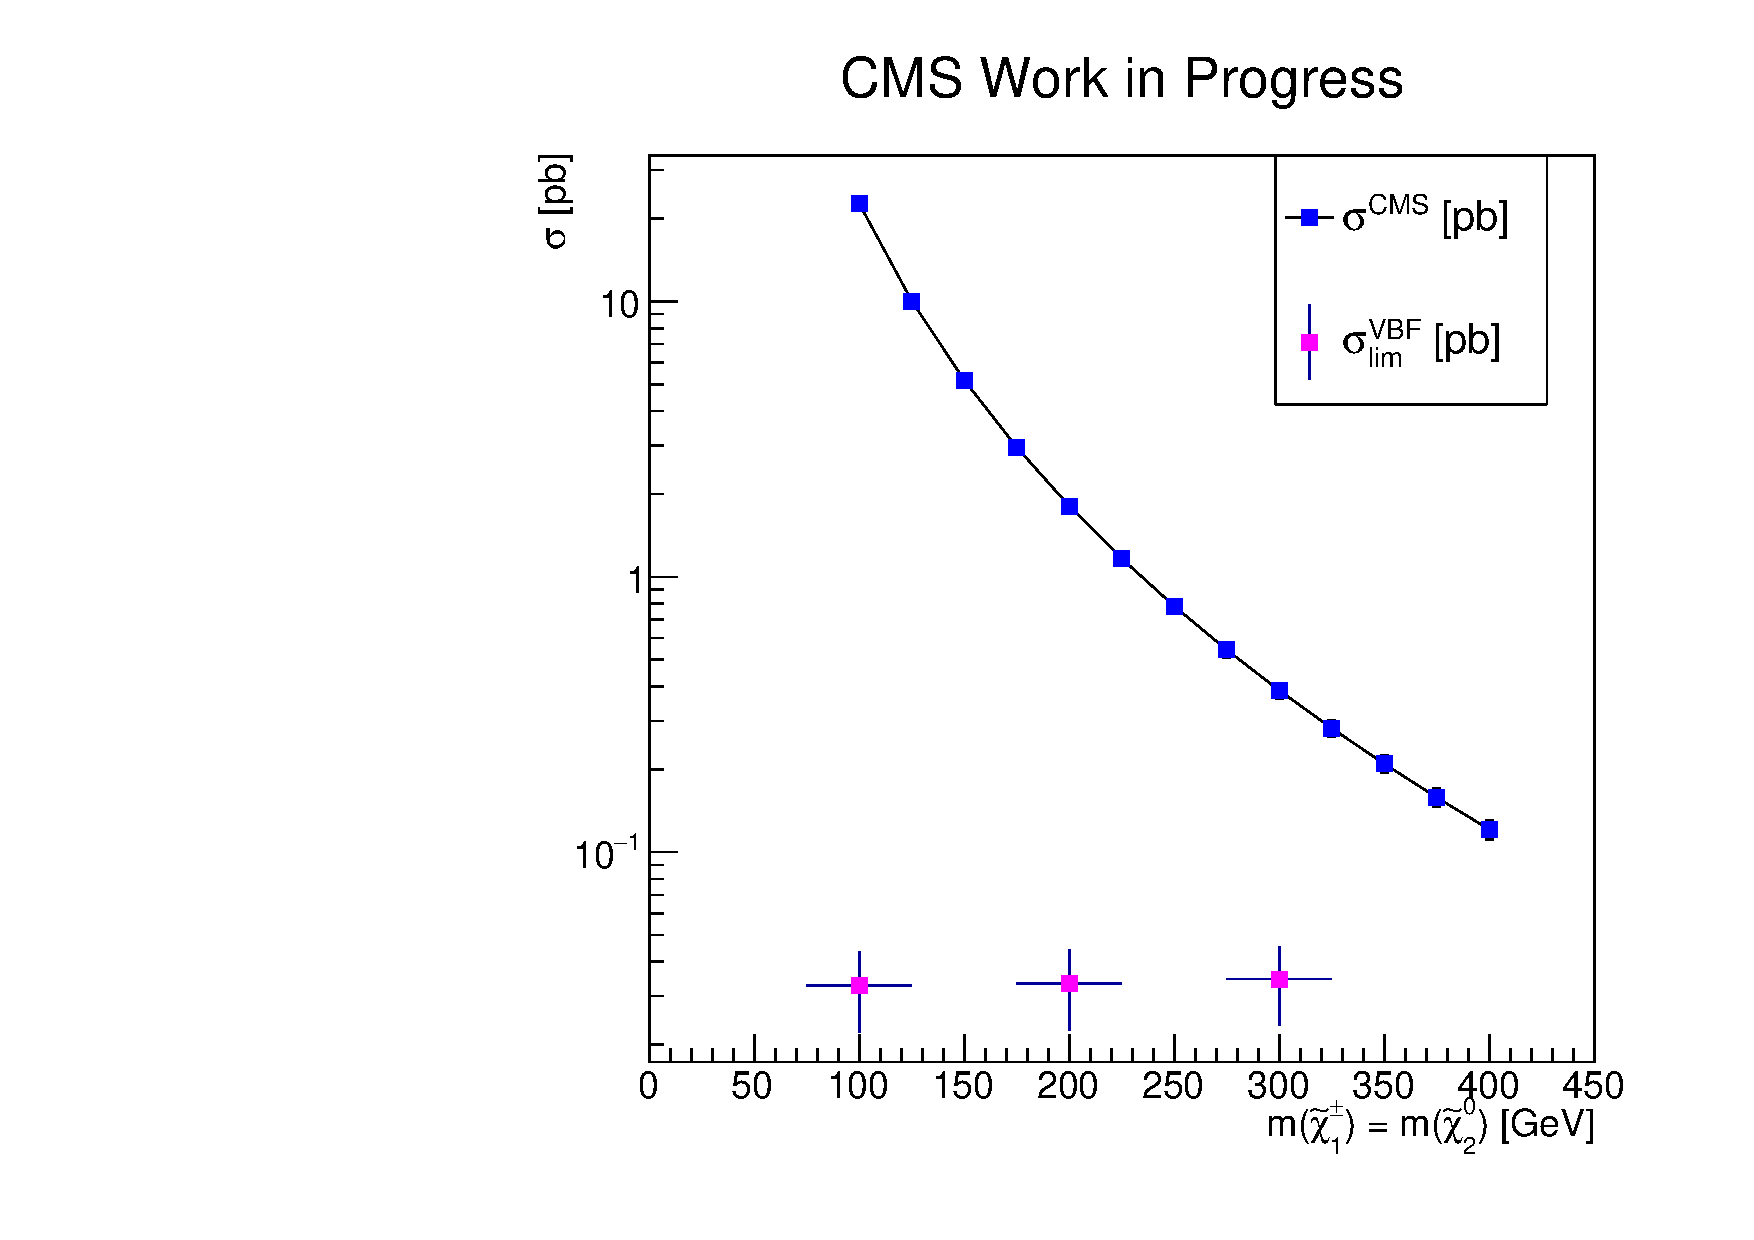
\includegraphics[width=0.75\textwidth]{analysis/pics/xsec_confront.pdf}
	\end{tabular}
	\caption{Comparison between the cross section limit given by this 13\tev study and official CMS cross sections calculated using the resummino code from B. Fuks et al with CTEQ6.6 and MSTW2008nlo90cl PDFs \cite{bib:SUSYCrossSections13TeVn2x1wino_13tev}.}
	\label{fig:xsec_confront_13tev}
\end{figure}


